\chapter{Abstract Factory \\
  \small{\textit{-- Evan Ciok, Sophia DiCuffa, Carson McManus}}
  \index{Chapter!AbstractFactory}
  \index{Abstract Factory}
  \label{Chapter::AbstractFactory}}

\section{Diagrams}

\href{https://github.com/dyc3/ssw345-group-assignments/blob/main/Figures/abstractFactory/figures-source.md}{View all diagrams in browser}

\begin{figure}[hp!]
  \centering
  \scalebox{0.25}{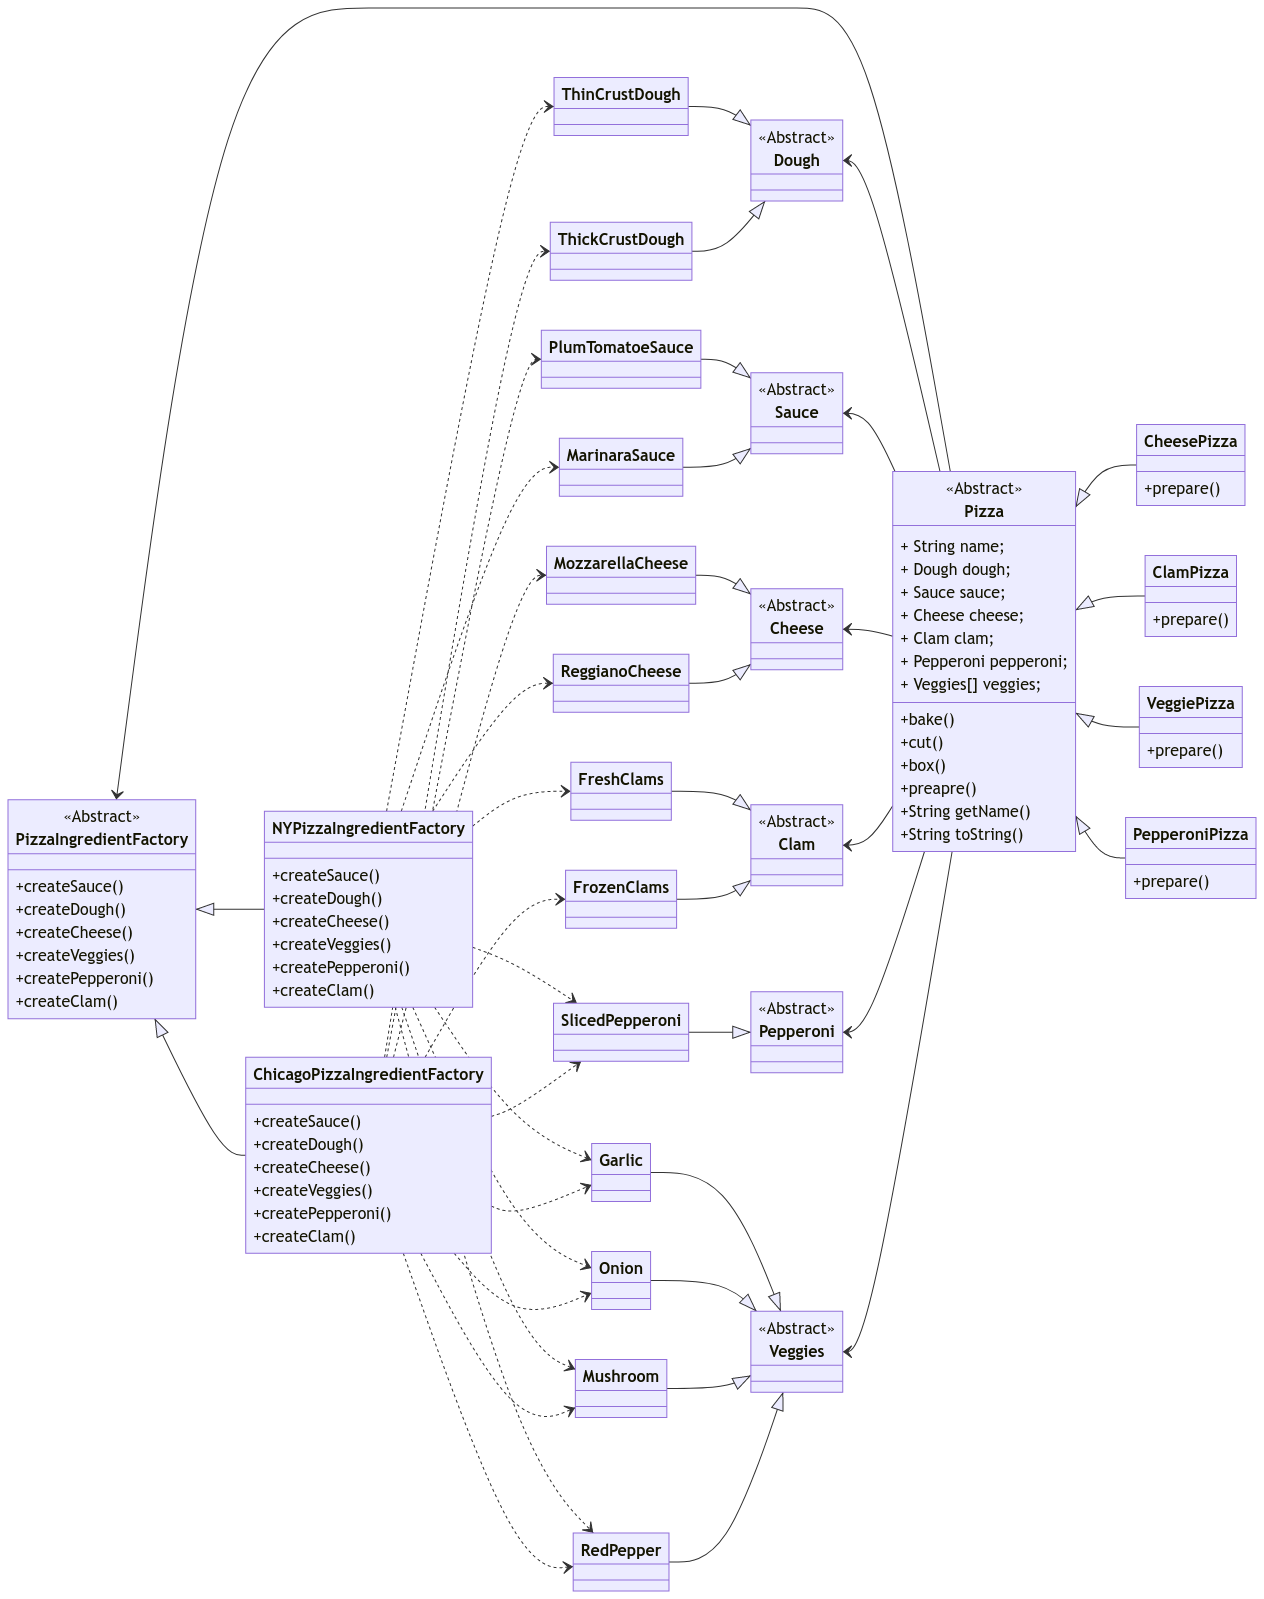
\includegraphics{Figures/abstractFactory/pizza.png}}
  \caption{\label{Figure::pizzadiagram} A class diagram for the pizzas.}
\end{figure}

\begin{figure}[hp!]
  \centering
  \scalebox{0.25}{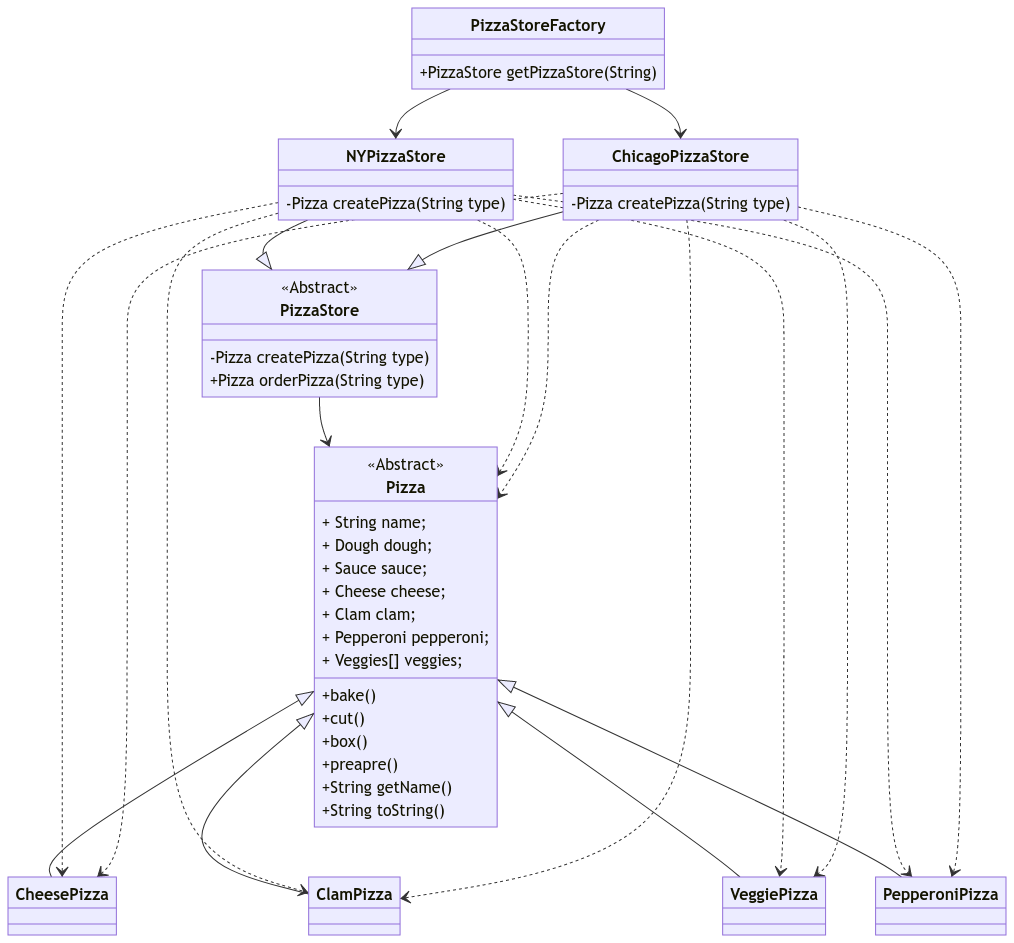
\includegraphics{Figures/abstractFactory/pizzastore.png}}
  \caption{\label{Figure::pizzastorediagram} A class diagram for the pizza stores.}
\end{figure}

\begin{figure}[hp!]
  \centering
  \scalebox{0.25}{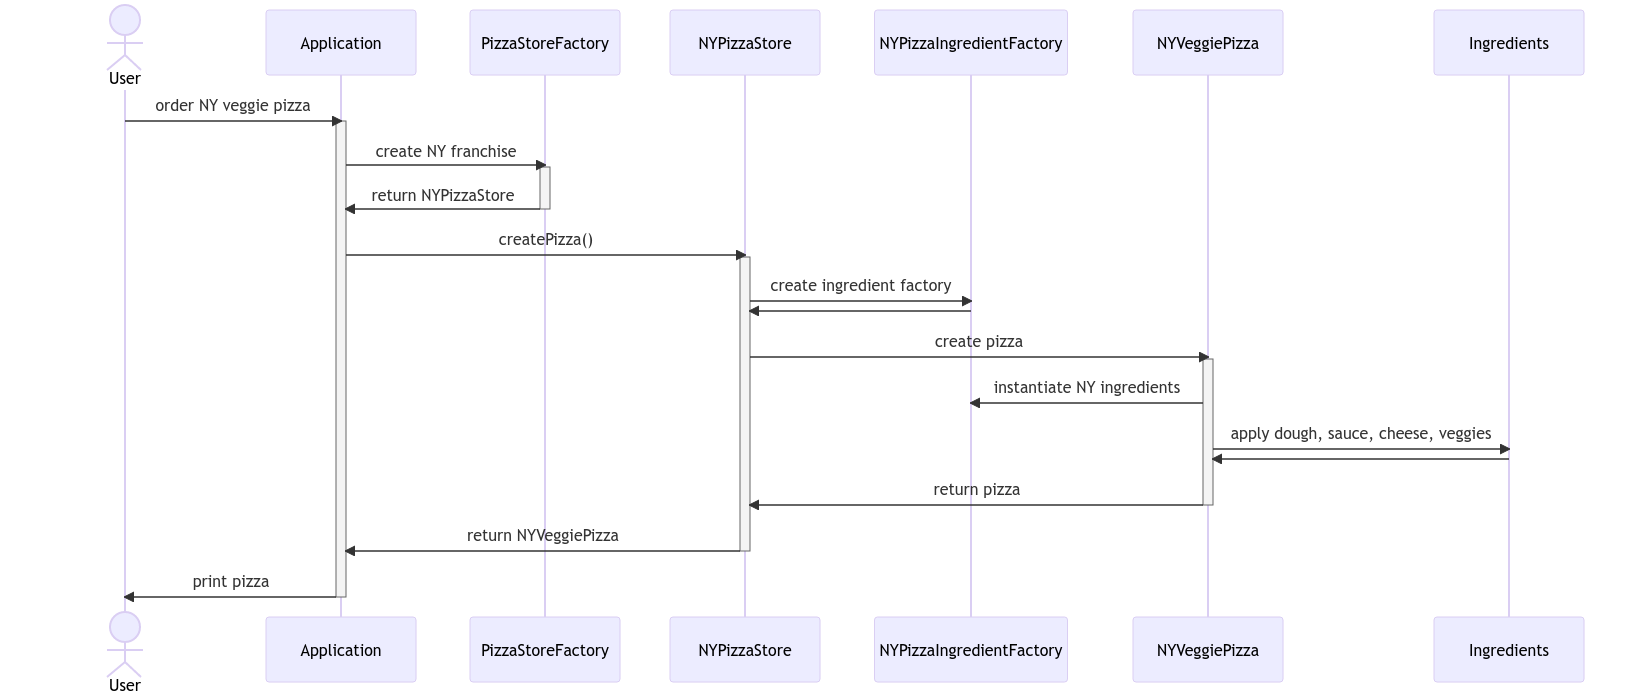
\includegraphics{Figures/abstractFactory/pizzaseq.png}}
  \caption{\label{Figure::pizzaseqdiagram} A sequence diagram for ordering a veggie pizza.}
\end{figure}

\pagebreak

\section{Code}

Code: \href{https://github.com/dyc3/ssw345-group-assignments}{github} (see abstract-factory-hw folder)

\subsection{Output}

The output of the program is shown in Figure \ref{Figure::pizzaoutput}.

\begin{figure}[hp!]
  \centering
  \scalebox{0.25}{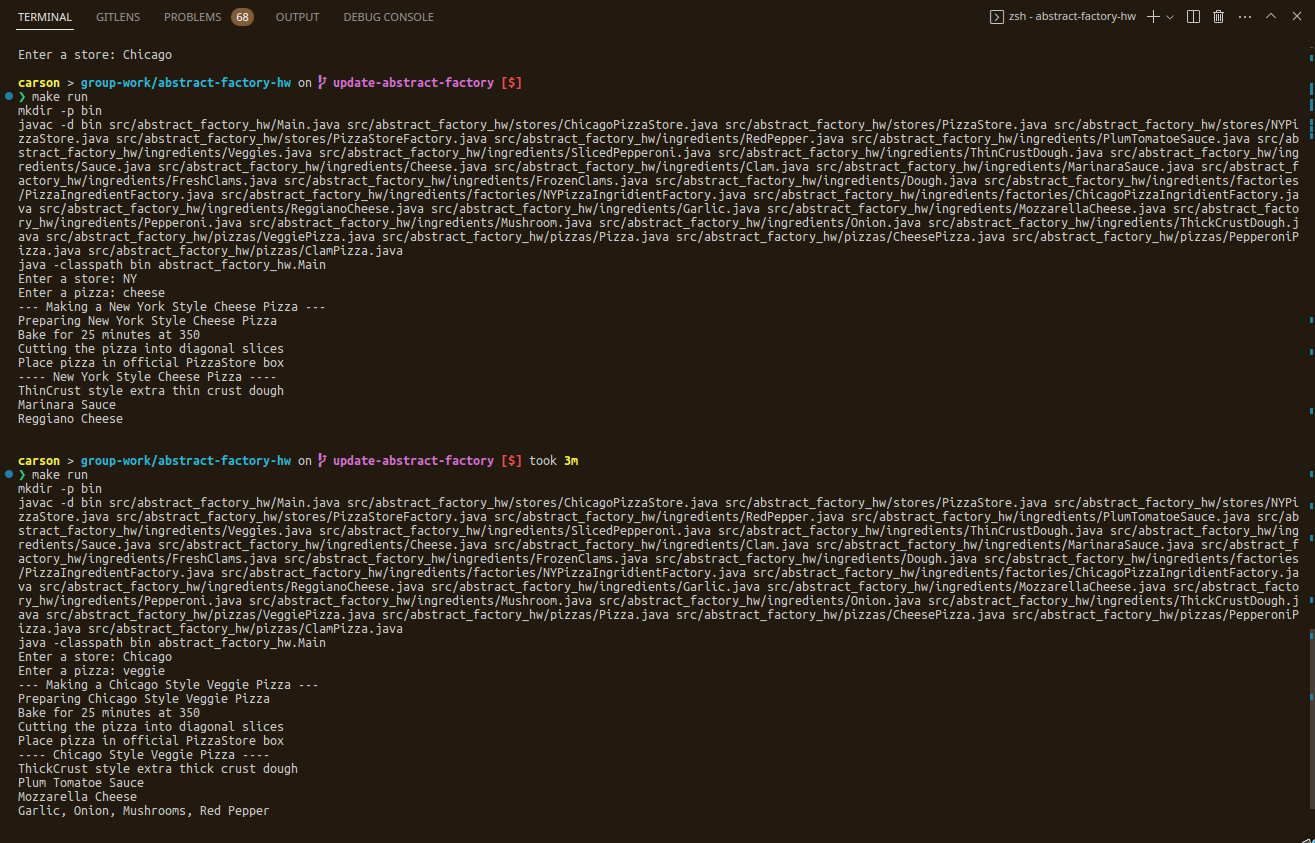
\includegraphics{Figures/abstractFactory/pizzaoutput.png}}
  \caption{\label{Figure::pizzaoutput} Example program outputs from the pizza program.}
\end{figure}